\documentclass[cn,11pt,chinese,black,toc=twocol]{elegantbook}
\title{利息理论}
\subtitle{made by \LaTeX{} }
\author{Icecream}
\cover{cover14.pdf}
% 本文档命令
\usepackage{tikz}
\usepackage{mathpazo} 
\usepackage{array}
\newcommand{\ccr}[1]{\makecell{{\color{#1}\rule{1cm}{1cm}}}}

\begin{document}
\def\angles#1{{%
		\vbox{\hrule height .2pt
			\kern 1pt
			\hbox{$\scriptstyle {#1}\kern 1pt$}%
		}\kern-.05pt \vrule width .2pt
}}
%
\maketitle
\tableofcontents

\chapter*{Introduction}
\markboth{Introduction}{Introduction}
保险精算研究的对象是年金,现金流和债券,年金的性质是研究现金流和债券的基础
\chapter{拓扑空间}
\begin{introduction}
	\item 开集
	\item 邻域
	\item 内点
	\item 稠密
\end{introduction}
\section{开集,闭集}
\begin{definition}{开集}
\noindent Let $(X, \mathcal{T})$ be any topological space. Then the members of $\mathcal{T}$ are said to be open sets.
\end{definition}
\begin{remark}
	开集和闭集不是一个相对概念,同一个成员可能同时开同时闭
\end{remark}
\begin{example}
	$\begin{array}{lll}  \text { Let } X=\{a, b, c, d, e, f\} \text { and }\end{array}$
	\[
	\tau_{1}=\{X, \emptyset,\{a\},\{c, d\},\{a, c, d\},\{b, c, d, e, f\}\}
	\]
	找出又开又闭的集合,只开,只闭的集合
\end{example}
\begin{remark}
	又开又闭的集合:$\{a\}$ \\
	只开:$\{c, d\}$
	只闭:$\{b,e,f\}$
\end{remark}
\begin{definition}{有限补拓扑}
	$\mathcal{T}_{f}=\left\{A \subset X | \quad A^{c} \text { 是 } X \text {的有限子集}\right\} \cup\{\emptyset\}$
\end{definition}
\begin{definition}{可数补拓扑}
	$\mathcal{T}_{c}=\left\{A \subset X | \quad A^{c} \text { 是 } X \text {的可数子集}\right\} \cup\{\emptyset\}$
\end{definition}
\begin{definition}{邻域}
\noindent $(X,\tau) ,A\subset X,x \in A$,
$\exists U \in \tau\rightarrow x \in U \subset A$
$x$为$A$的内点,$A$为$x$的邻域
\end{definition}
\begin{definition}{内点,内部}
\noindent	 已知拓扑空间 $X, x \in X, A \subseteq X,$ 若
	\[
	\exists x \text { 的邻域 } U, \text { s.t. } \quad U \subseteq A
	\]
	则称 $x$ 是 $A$ 的 内点 $. A$ 的全体内点记为 $A^{\circ},$ 称为 $A$ 的内部 $(\text { interior })$
\end{definition}
\begin{property}
(1). 若 $A \subset B,$ 则 $A^{\circ} \subset B^{\circ}$ \\
(2). $A^{\circ}=\bigcup\{U \subset X | U \text { 是 } X \text { 的开集且 } U \subset A\},$ 因此 $A$ 的内部 $A^{\circ}$ 是包含在
$A$ 中最大的开集;\\
(3). $A$ 是开集 $\Longleftrightarrow A=A^{\circ}$\\
$(4) \cdot(A \cap B)^{\circ}=A^{\circ} \cap B^{\circ}$ \\
$(5) .(A \cup B)^{\circ} \supset A^{\circ} \cup B^{\circ}$ \\
\end{property}
\begin{definition}{聚点}
\noindent 设 $A$ 是拓扑空间 X 的子集, $x \in X .$ 如果 $x$ 的任何一个邻域 $U,$ 都
有 $U \cap(A \backslash\{x\}) \neq \emptyset,$ 称 $x$ 为 $A$ 聚点. \\$A$ 的所有聚点的集合称为 $A$ 的导集,记
作 $d(A) .$  \\称集合 $\bar{A}=A \cup d(A)$ 为 $A$ 的闭包.
\end{definition}
\begin{theorem}
\noindent $x \in \bar{A} \Longleftrightarrow x$ 的任意邻域与 $A$ 相交都不空.
\end{theorem}
\begin{theorem}
\noindent A 是拓扑空间 X 的稠密子集$\Longleftrightarrow$ X 的每个非空开集与 A 相交非空
\end{theorem}
\begin{definition}{稠密}
\noindent 拓扑空间 X 的子集 A 称为稠密的,如果 $\bar{A}=X .$ 如果 $X$ 有一个
可数的稠密子集,则称 X 是可分空间
\end{definition}
\begin{exercise}
设 $\mathbb{Z}+$ 是全体正整数的集合,令 表示满足如下条件的集合$U$构成的
集族 $\mathcal{T}$\\
“若 $n \in U,$ 则 $\mathrm{n}$ 的每个因数都在 $\mathrm{U}$ 中"
是$\mathbb{Z}+$的一个拓扑。\\
(a). 设集合 $B=\{2,5\},$ 求: $d(B)$

\end{exercise}
\chapter{等额年金}
\begin{introduction}
	\item 每年支付m次的年金
	\item 连续支付的等额年金
\end{introduction}
\section{符号一览}
\noindent$a_{\angles{n}},s_{\angles{n}}$\\	$\ddot{a}_{\angles{n}}$\\$\ddot{s}_{\angles{n}}$
\section{等额年金}
\begin{definition}{年金的终值与现值}
\noindent $a_{\angles{n}},s_{\angles{n}}$\\
$s_{\angles{n}}=a_{\angles{n}}(1+i)^{n}=\frac{(1+i)^{n}-1}{i}$
\end{definition}
\begin{definition}{Accumulated Value of an $n$ -Payment Annuity-Immediate of 1 Per Period}

	The symbol $s_{\angles{n}}$ denotes the accumulated value, at the time of (and including) the final payment of a series of $n$ payments of 1 each made at equally spaced intervals of time, where the rate of interest per payment period is $i$
	$\begin{aligned}
	s_{\angles{n}} &=(1+i)^{n-1}+(1+i)^{n-2}+\cdots+(1+i)+1 \\
	&=\sum_{t=0}^{n-1}(1+i)^{t}=\frac{(1+i)^{n}-1}{i}
	\end{aligned}$
\end{definition}
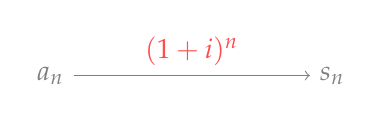
\begin{tikzpicture}
\draw [color=black!50,->](0,0) node[left]{$a_{\angles{n}}$}-- node [color=red!70,pos=0.5,above,sloped]{$(1+i)^n$}(3,0) node[right]{$s_{\angles{n}}$};
    \end{tikzpicture} \\
\noindent $a_{\angles{n}}=v+v^2+v^3+\dots+v^n=\frac{1-v^n}{i}=\frac{1-\frac{1}{(1+i)^n}}{i}=\frac{1-v^n}{\frac{1}{v}-1}$\\
\begin{lstlisting}[language={python}]
#wolframalpha
(1-(1/(1+i)^n))/i=(1-v^n)/(1/v-1)
\end{lstlisting}
$\ddot{a}_{\angles{n}}=\frac{1-v^n}{d}$ \\
$s_{\angles{n}}=a_{\angles{n}}(1+i)^{n}=\frac{(1+i)^{n}-1}{i}$\\
$\ddot{s}_{\angles{n}}=\ddot{a}_{\angles{n}}(1+i)^{n}=\frac{(1+i)^{n}-1}{d}$
\begin{property}
$1=i{a}_{\angles{n}}+v^n$
\end{property}
 \begin{definition}{每年支付m次年金}
 \noindent ${a}_{\angles{n}}^{\(m\)}=\frac{1-v^n}{i^{(m)}}$ 
 \end{definition}
 
\chapter{紧致性}
\begin{definition}{cover}
A collection $\mathcal{A}$ of subsets of a space $X$ is said to cover $X,$ or to be a covering of $X,$ if the union of the elements of $\mathcal{A}$ is equal to $X .$ It is called an open covering of $X$ if its elements are open subsets of $X$
\end{definition}
\begin{definition}{compact}
A space $X$ is said to be compact if every open covering $\mathcal{A}$ of $X$ contains a finite subcollection that also covers $X$
\end{definition}
\begin{theorem}
Every closed subspace of a compact space is compact.
\end{theorem}
\chapter{收益率}
\begin{introduction}
	\item 收益率
	\item 再投资
	\item 基金
\end{introduction}
\section{收益率}
净现值
\\收益率法
\section{基金的利息度量}
\begin{definition}{Dollar-Weighted Return For a One-Year Period}
\noindent	Suppose the following information is known:
	(i) the balance in a fund at the start of the year is $A$ \\
	(ii) for $0<t_{1}<t_{2}<\cdots<t_{n}<1,$ the net deposit at time $t_{k}$ is amount $C_{k}$ (positive for a net deposit, negative for a net withdrawal), and \\
	(iii) the balance in the fund at the end of the year is $B$
	Then the net amount of interest earned by the fund during the year is $I=B-\left[A+\sum_{k=1}^{n} C_{k}\right],$ and the dollar-weighted rate of return earned by the fund for the year is
	\[
	\frac{I}{A+\sum_{k=1}^{n} C_{k}\left(1-t_{k}\right)}
	\]
\end{definition}
\begin{remark}
	$(Ia)_{\angles{n}}=\frac{\ddot{a}_{\bar{n}}-n v^{n}}{i}$
\end{remark}
\begin{definition}{Time-Weighted Return For a One-Year Period}
\noinent Suppose the following information is known:\\
	(i) the balance in a fund at the start of the year is $A$\\
	(ii) for $0<t_{1}<t_{2}<\cdots<t_{n}<1,$ the net deposit at time $t_{k}$ is amount $C_{k}($ positive for a net deposit, negative for a net withdrawal)\\
	(iii) the value of the fund just before the net deposit at time $t_{k}$ is $F_{k},$ and\\
	(iv) the balance in the fund at the end of the year is $B$
	The time-weighted return rate earned by the fund for the year is
	\[
	\left[\frac{F_{1}}{A} \times \frac{F_{2}}{F_{1}+C_{1}} \times \frac{F_{3}}{F_{2}+C_{2}} \times \cdots \times \frac{F_{k}}{F_{k-1}+C_{k-1}} \times \frac{B}{F_{k}+C_{k}}\right]-1
	\]	
\end{definition}	
\section{再投资}


\section{基金}
\chapter{债务偿还方法}
\begin{introduction}
	\item 等额分期偿还
	\item 等额偿债基金
	\item 变额分期偿还
\end{introduction}
\section{分期偿还法}
\subsection{等额分期偿还}
\noinent 每次偿还的金额:$R=\frac{L_0}{a_{\angles{n}}}$\\
未偿还本金:$L_k=Ra_{\angles{n-k}}=L_0(1+i)^k-Rs_{\angles{k}}$\\
\\ 支付的本金:
支付的利息:$I_k=iL_{k-1}=iRa_{\angles{n-k+1}}=R(1-v^{n-k+1})$\\
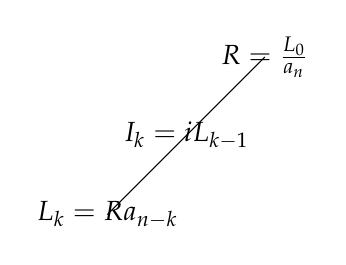
\begin{tikzpicture}
\draw (1,1) node{$L_k=Ra_{\angles{n-k}}$} -- (2,2) node{$I_k=iL_{k-1}$}-- (3,3) node{$R=\frac{L_0}{a_{\angles{n}}}$};
\end{tikzpicture}
\begin{exercise}
贷款一笔钱,n年内等额分期付款,每年末还一次,偿还金额是X,第一年利息是604RMB,第三年是593.75,第五年利息是582.45,计算X
\end{exercise}
\begin{note}
支付的利息:$I_k=iL_{k-1}=iRa_{\angles{n-k+1}}=R(1-v^{n-k+1})$
\end{note}
\begin{exercise}
按年实际利率i偿还一笔 1000 元的贷款。已知:\\
(1)在第6年末偿还第一笔款项\\
(2)然后每年未等额偿还一次在第15年末可以偿清这笔贷款(即一共偿还 10 次)\\
(3)在第10年末的付款结束后。未偿还本金余额为 908.91 元\\
试计算第5年末的未偿还本金余额
\end{exercise}
\begin{solution}
设等额付款金额为 $R: Ra_{\angles{5}i}=908.81, Ra_{\angles{10}}=1000(1+i)^5 \\
故第5年末的未归还本金为 $1000 \times(1+i)^{5}=1510.6$ 元
\end{solution}
\section{等额偿债基金}
区别:偿还本金采用不同的计息方式\\
$$D=\frac{L_0}{s_{\angles{n}j}}$$\\
$$R=I+D$$\\
$$L_k=L_0-Ds_{\angles{n}j}$$
\chapter{债务价值分析}
\section{符号一览}
\noindent $P:$ 债券价格 (bond price) \\
$i$ :债券的到期收益率(yield-to-maturity rate),即投资人购买债券者购买债券所要求的收益率\\
$F :$ 债券的面值 (par value,face amount, nominal value),即债券到时支付给债券持有人的金额,也称为票面价值或到期值\\
$r:$ 债券的息票率 (coupon rate per payment period)\\
$rF$ 息票收入 \\
$i_{c}:$ 债券的当期收益率: $i_{c}=\frac{r F}{P}$\\
$C :$ 债券的偿还值 (redemption payment),通常等于侦券面值F\\
$n$ : 息票的支付次数 (number of coupon payments)\\
$g:$ 债券的修正息票率, $g=\frac{r F}{C}$\\
债券定价原理:到期偿还值+债券未来息票
$$P=rFa_{\angles{n}}+Cv^n$$
\chapter{利率风险}
\begin{definition}{利息力}
\noindent		设可积函数连续可导,则称
\[
\delta_{t}=\frac{a^{\prime}(t)}{a(t)}=[\ln a(t)]^{\prime}
\]
为时刻 t 的利息力
		\end{definition}
		\\ 衡量利息增长速率与利息本身大小的比值
		很有意思的是,我们把t当做横坐标的时候,相当于t是定下来的,以这个为标准来用利息力来计算累积函数
		$$\int_{0}^{t} \delta_{s} d s=\int_{0}^{t} \frac{a^{\prime}(s)}{a(s)} d s=\int_{0}^{t}[\ln a(s)]^{\prime} d s=\ln a(t)$$
\section{Macaulay duration}
	\begin{definition}{Macaulay duration}
$$D_{\text {麦 }}=\frac{\sum_{t>0} t \cdot R_{t} e^{-\delta t}}{\sum_{t>0}  \cdot R_{t} e^{-\delta t}}$$
\end{definition}
\begin{note}
一笔 $n$ 年期贷款,年实际利率为 $i,$ 按年等额分期偿还,求该笔贷款的麦考利久期。
\end{note}
\begin{solution}
$$\begin{aligned}
D_{\text {麦 }} &=\frac{\sum\limits_{t>0} t \cdot R(1+i)^{-t}}{\sum\limits_{t>0} R(1+i)^{-t}}=\frac{(I a)_{\angles{n }}}{a_{\angles{n }}}} \\
&=\frac{\ddot{a}_{\angles{n}}-n v^{n}}{i \cdot a_{\angles{n }}}=\frac{(1+i) a_{\angles{n }}}{i \cdot a_{\angles{n }}}-\frac{n v^{n}}{i \cdot \frac{1-v^{n}}{i}} \\
&=\frac{1+i}{i}-\frac{n}{(1+i)^{n}-1}
\end{aligned}$$
\end{solution}
\subsection{修正久期}
\begin{definition}{修正久期}
$$D=\frac{D_{\text {麦 }}}{1+\frac{y}{m}}$$
\end{definition}
\begin{note}
	债券面值为F,期限为n,到期时按面值偿还,年息票率为r,到期收益率r,求$D_{\text {麦 }$\\
		$$D_{\text {麦 }}=\frac{\sum_{t=1}^{n}tv^trF+nv^nF}{\sum_{t=1}^{n}rFv^t+v^nF}$$
		$$=\frac{\sum_{t=1}^{n}tv^tr+nv^n}{\sum_{t=1}^{n}rv^t+v^n}$$
\end{note}
\begin{exercise}
某 2 年期债券的面值为 1000 元,年息票率为 8%,每半年末支付一次利息,债券到期按面值偿还。该债券每半年复利一次的到期收益率为4%,请计算该债券的修正久期
\end{exercice}
\begin{solution}
该债券的价格为
$$P=2 \times 40 a_{\angles{2}4 \%}^{(2)}+1000 \times(1+4 \% / 2)^{-4}=1076.16(\text { 元 })
$$
麦考利久期为
$$D_{\text {麦 }}=\frac{\sum_{t>0} t \cdot R_{t}(1+i)^{-t}}{P}=\frac{2036.19}{1076.16}=1.89$$
修正久期:$$D=\frac{D_{\text {麦 }}}{1+i^{(2)} / 2}=\frac{1.89}{1+4 \% / 2}=1.86$$
\end{solution}
\end{document}
